\documentclass{article}

% NeurIPS 2025 style
\usepackage[final]{neurips_2025}

\usepackage[utf8]{inputenc}
\usepackage[T1]{fontenc}
\usepackage{hyperref}
\usepackage{url}
\usepackage{booktabs}
\usepackage{amsfonts}
\usepackage{nicefrac}
\usepackage{microtype}
\usepackage{xcolor}
\usepackage{graphicx}
\usepackage{algorithm}
\usepackage{algorithmic}
\usepackage{amsmath}
\usepackage{amssymb}
\usepackage{subcaption}
\usepackage{multirow}
\usepackage{tikz}
\usepackage{pgfplots}
\pgfplotsset{compat=1.18}
\usetikzlibrary{shapes,arrows,positioning,calc}

\title{Neural Steering: Practical Circuit Discovery and Control \\ in Language Models}

\author{%
  Anonymous Authors \\
}

\begin{document}

\maketitle

\begin{abstract}
We present a practical, standalone toolkit for discovering and steering neuron-level circuits in large language models.
Building on Relevance Propagation (RelP) attribution in the neuron basis, we show that \emph{as few as 100--200 MLP neurons} form complete, faithful circuits for diverse tasks.
Our toolkit requires only PyTorch and Hugging Face Transformers---no sparse autoencoder training, no control vector computation, no gradient integration.
A single forward-backward pass identifies the causal circuit; modifying those neurons' activations at inference steers model behavior without disrupting unrelated capabilities.
We demonstrate: (1)~factual recall circuits where ablating the top neuron eliminates the correct answer on held-out prompts, (2)~contrastive refusal circuits where zeroing ${\sim}200$ neurons converts safety refusal to full compliance while leaving benign prompts unchanged, (3)~faithfulness curves matching the reference implementation with 2\% of neurons achieving $f{=}0.74$ (simple) and $f{=}0.90$ (nounpp) on subject-verb agreement, (4)~edge attribution revealing an hourglass architecture in which a single neuron serves as both major source hub and target hub, and (5)~zero-code cross-model generalization to Qwen2.5-7B and Mistral-7B.
We also connect neuron circuits to super weight neurons via edge attribution, finding that anomalously large weight magnitudes in early layers act as universal infrastructure neurons detectable across tasks and models.
Our toolkit and all experiments are released as a single-file Python module.
\end{abstract}


%% ===================================================================
\section{Introduction}
\label{sec:intro}
%% ===================================================================

Understanding the internal computations of large language models (LLMs) remains a core problem in AI safety and interpretability.
The dominant approach---mechanistic interpretability---seeks to reverse-engineer the algorithms implemented by neural networks by identifying \emph{circuits}: sparse subsets of model components that are jointly responsible for a particular behavior \citep{conmy2023acdc, wang2023ioi, elhage2022toy}.

Prior work on circuit discovery has primarily operated in one of three representational bases: the \emph{residual stream} (activation patching and path patching \citep{meng2022rome, goldowskydill2023localizing}), the \emph{attention head} basis (circuit-level analysis of attention patterns \citep{wang2023ioi}), or the \emph{sparse autoencoder (SAE) feature} basis (learning interpretable directions via dictionary learning \citep{cunningham2023sae, bricken2023monosemanticity, templeton2024scaling, marks2024sparse}).
Each approach has fundamental trade-offs.
Activation patching requires $O(n)$ forward passes per component and struggles to scale.
SAEs require expensive unsupervised training, face the dictionary--granularity dilemma, and can miss features not in the learned dictionary.

Recent work by \citet{arora2025circuits} demonstrates an alternative: circuits are \emph{sparse in the neuron basis}.
Using Relevance Propagation (RelP) \citep{achtibat2024relp, bach2015pixel} with three linearization rules adapted for transformer MLP blocks, the authors show that roughly 100--200 MLP neurons suffice to explain model behavior on factual recall and syntactic agreement tasks, with RelP attribution achieving 0.956 correlation with activation patching at a fraction of the computational cost.

In this paper, we build on this foundation and present a \emph{practical, standalone toolkit} for neuron-level circuit discovery and steering.
Our contributions are:

\begin{enumerate}
    \item \textbf{A dependency-light toolkit.} A single-file Python module (\texttt{neuron\_steer.py}) implementing RelP attribution, circuit selection, neuron-level steering, contrastive discovery, edge attribution, and faithfulness evaluation. No SAE training, no external interpretability libraries.

    \item \textbf{Contrastive circuit discovery.} A method for finding behavior-specific neuron circuits (e.g., refusal, tone, style) by contrasting MLP activations between two prompt sets, enabling steering of high-level behaviors beyond factual recall.

    \item \textbf{Edge attribution and hourglass architecture.} A procedure for tracing neuron-to-neuron information flow within circuits, revealing that circuits exhibit an hourglass topology with bottleneck neurons that serve as both major source hubs (high fan-out) and target hubs (high fan-in).

    \item \textbf{Universal neuron detection and super weight connection.} An automated procedure for detecting universal neurons that fire across all tasks, and a connection between these neurons and super weights \citep{zhong2024superweights}---anomalously large weight magnitudes in early layers that act as task-agnostic infrastructure.

    \item \textbf{Cross-model generalization.} Demonstration that the same code, with \emph{zero modifications}, discovers and steers circuits in Llama-3.1-8B, Qwen2.5-7B, and Mistral-7B.
\end{enumerate}


%% ===================================================================
\section{Background}
\label{sec:background}
%% ===================================================================

\subsection{Relevance Propagation for Transformers}

Layer-wise Relevance Propagation (LRP) \citep{bach2015pixel} decomposes a model's output prediction into per-input-feature relevance scores by propagating relevance backward through the network using local redistribution rules.
AttnLRP \citep{achtibat2024relp} extends LRP to transformers.
\citet{arora2025circuits} demonstrate that AttnLRP achieves 0.956 Pearson correlation with activation patching on circuit discovery benchmarks while requiring only a single forward-backward pass.

\citet{arora2025circuits} apply AttnLRP with three modifications specific to the Llama MLP architecture, which we describe in Section~\ref{sec:method}.
Their key finding is that circuits identified in the \emph{neuron basis} (individual MLP intermediate activations) are remarkably sparse: ${\sim}100$--$200$ neurons explain complete task circuits, compared to thousands of SAE features.


\subsection{Contrastive Activation Addition}

Representation Engineering \citep{zou2023representation} and Contrastive Activation Addition (CAA) \citep{rimsky2024steering} steer model behavior by computing a \emph{control vector}: the mean difference in residual stream activations between positive and negative prompt sets.
Adding this vector during inference shifts model behavior along the identified direction.
While effective, CAA operates in the full residual stream and does not decompose to individual neurons, making it difficult to understand \emph{which} computations are being modified.

\subsection{Super Weights}

\citet{zhong2024superweights} identify \emph{super weights}: individual weight matrix entries in early transformer layers with magnitudes 1000--5000$\times$ larger than typical entries.
These parameters are critical for model function---zeroing a single column can collapse model output.
Their role within the broader circuit structure of LLMs has not been previously characterized.


%% ===================================================================
\section{Method}
\label{sec:method}
%% ===================================================================

Our toolkit implements three linearization rules that convert the non-linear components of transformer MLP blocks into linear approximations suitable for gradient-based attribution.
These rules match the implementation of \citet{arora2025circuits}, verified against their released codebase.

\subsection{The Three LRP Rules}
\label{sec:lrp_rules}

\paragraph{Rule 1: LN-rule (RMSNorm Linearization).}
RMSNorm computes $y = x \cdot w \cdot \text{rsqrt}(\text{mean}(x^2) + \epsilon)$, where $w$ is the learned weight vector.
The LN-rule treats the normalization coefficient $c = w \cdot \text{rsqrt}(\text{mean}(x^2) + \epsilon)$ as a \emph{detached constant} in the backward pass: the forward produces the correct normalized value, but the backward pass computes $\frac{\partial \mathcal{L}}{\partial x} = \frac{\partial \mathcal{L}}{\partial y} \cdot c_{\text{detach}}$.
This preserves the per-token scaling (unlike a pure identity rule) while eliminating the non-linear interaction between input magnitude and gradient:

\begin{equation}
    \textsc{Forward:} \quad y = x \cdot c, \qquad
    \textsc{Backward:} \quad \nabla_x = \nabla_y \cdot \text{sg}(c)
\label{eq:ln_rule}
\end{equation}

where $\text{sg}(\cdot)$ denotes stop-gradient (detach).

\paragraph{Rule 2: AH-rule (Eager Attention).}
Flash Attention and Scaled Dot-Product Attention (SDPA) compute attention in fused kernels that do not expose intermediate gradients to PyTorch's autograd.
The AH-rule replaces these with \emph{eager} attention: explicit matrix multiplications $QK^\top / \sqrt{d_k}$, softmax, and value projection.
This ensures gradient flows through all attention components, including $Q$ and $K$ projections:

\begin{equation}
    A = \text{softmax}\left(\frac{QK^\top}{\sqrt{d_k}}\right), \qquad O = AV
\end{equation}

Crucially, the original TransluceAI implementation does \emph{not} zero $Q/K$ gradients (despite the class name \texttt{NoQKGradAttention}); it simply ensures non-fused computation.
We match this behavior by setting \texttt{config.\_attn\_implementation = "eager"}.

\paragraph{Rule 3: Half-rule (Shapley Attribution for Gated MLPs).}
Llama-family models use a gated MLP: $h = \sigma(\text{gate}(x)) \cdot \text{up}(x)$, where $\sigma$ is SiLU.
The elementwise multiply of two input-dependent factors creates an attribution problem: how much credit should each factor receive?

The Half-rule applies Shapley value theory \citep{shapley1953value}: each factor receives 50\% of the gradient.
The sigmoid component of SiLU is also detached, linearizing SiLU to a scaled identity.
Formally, with $g = \text{gate}(x)$ and $u = \text{up}(x)$:

\begin{align}
    \hat{g} &= g \cdot \text{sg}(\sigma(g))  && \text{(linearized SiLU)} \\
    h &= \textsc{HalfRule}(\hat{g}, u) && \text{(Shapley multiply)}
\end{align}

where the custom autograd function distributes gradients:
\begin{equation}
    \nabla_{\hat{g}} = \nabla_h \cdot u \cdot 0.5, \qquad \nabla_u = \nabla_h \cdot \hat{g} \cdot 0.5
\end{equation}

The intermediate activation $h$ (input to $\texttt{down\_proj}$) is the \emph{neuron activation} that we attribute and steer.

\subsection{Attribution Pipeline}
\label{sec:pipeline}

Given a prompt and target token, we compute per-neuron attribution scores:

\begin{algorithm}[h]
\caption{Neuron Circuit Discovery via RelP}
\label{alg:discovery}
\begin{algorithmic}[1]
\REQUIRE Model $M$, prompt $x$, target token $t$, selection threshold $\tau$
\STATE Apply LRP rules: RMSNorm $\to$ LinearizedRMSNorm, attention $\to$ eager, MLP $\to$ LinearizedMLP
\STATE Forward pass: $\ell_t = \text{logit}_t(M(x))$
\STATE Backward pass: $\nabla \ell_t$ through linearized model
\STATE For each layer $l$, position $p$, neuron $n$: $a_{l,p,n} = \nabla_{h_{l,p,n}} \ell_t \cdot h_{l,p,n}$
\STATE Filter: remove blacklisted (universal) neurons, BOS position
\STATE Select: keep neurons where $|a_{l,p,n}| \geq \tau \cdot |\ell_t|$
\RETURN Circuit $C = \{(l, p, n, a_{l,p,n})\}$
\end{algorithmic}
\end{algorithm}

The attribution score $a_{l,p,n} = \text{grad} \times \text{activation}$ captures how much each neuron's current activation contributes to the target logit.
This is computed in a single forward-backward pass, compared to $O(n)$ forward passes for activation patching.

\paragraph{Selection methods.}
We support three selection strategies: (1)~\textsc{Top-k}: select the $k$ neurons with largest $|a|$; (2)~\textsc{Percentage}: keep neurons with $|a| \geq \tau \cdot |\ell_t|$ (matching TransluceAI's default of $\tau = 0.005$); (3)~\textsc{Cumulative threshold}: keep neurons until cumulative $|a|$ exceeds $\tau$ fraction of total attribution.

\paragraph{Backward from target logit alone.}
Following \citet{arora2025circuits}, we backward from the target token's logit $\ell_t$ directly, not from a logit difference $\ell_t - \ell_{cf}$.
The percentage threshold is relative to $|\ell_t|$, ensuring consistent circuit size across prompts.

\subsection{Universal Neuron Detection and Blacklisting}
\label{sec:blacklist}

Some MLP neurons fire strongly across \emph{all} prompts regardless of content.
These universal neurons appear in the top attribution for any task and inflate circuit sizes without contributing task-specific information.
\citet{arora2025circuits} provide a hard-coded blacklist for Llama-3-8B (12 neurons).

We implement an automated detection procedure: run $N$ diverse prompts, collect top-$k$ activated neurons at each layer, and flag neurons appearing in $\geq 80\%$ of prompts as universal.
For Llama-3.1-8B, this detects the known 12 neurons plus 2--5 additional ones.
For new architectures (Qwen, Mistral), it provides the first blacklist without manual analysis.

\subsection{Contrastive Circuit Discovery}
\label{sec:contrastive}

For behavioral features without clean target/counterfactual token pairs (e.g., refusal, sycophancy, creativity), we introduce a contrastive discovery method:

\begin{enumerate}
    \item Collect last-token MLP activations for positive prompts (exhibiting target behavior) and negative prompts (not exhibiting it).
    \item Compute per-neuron mean activation difference: $\delta_n = \bar{a}_n^{+} - \bar{a}_n^{-}$.
    \item Select top-$k$ neurons by $|\delta_n|$.
\end{enumerate}

This bypasses RelP entirely and operates on raw activations, making it applicable to any behavior expressible as a prompt contrast.

\subsection{Edge Attribution}
\label{sec:edges}

To understand information flow \emph{within} circuits, we compute neuron-to-neuron edge weights.
For each target neuron $t$ in the circuit (top-$k$ by attribution), we backward from $t$'s activation through the linearized model and read gradients at all source neurons in earlier layers:

\begin{equation}
    w_{s \to t} = \frac{\partial h_t}{\partial h_s} \cdot h_s
\end{equation}

This produces a directed graph $G = (V, E)$ where $V$ is the circuit neurons and $E$ are weighted edges representing attribution flow.
We analyze this graph for:
\begin{itemize}
    \item \textbf{Source hubs}: neurons with high fan-out (influence many downstream neurons).
    \item \textbf{Target hubs}: neurons with high fan-in (receive influence from many upstream neurons).
    \item \textbf{Bottleneck neurons}: neurons that are both source and target hubs, forming the ``narrow waist'' of an hourglass architecture.
\end{itemize}

\subsection{Super Weight Detection via Edge Attribution}
\label{sec:superweights}

Super weights \citep{zhong2024superweights} are anomalously large weight parameters in early transformer layers.
We detect their signature in circuit edge graphs: a source neuron is flagged as a super weight if its mean $|$edge weight$|$ exceeds $\rho \times$ the median across all source neurons (default $\rho = 10$).
By running edge attribution on multiple tasks (factual recall and refusal) and taking the \emph{intersection}, we identify neurons that are universal infrastructure rather than task-specific.

\subsection{Steering via Activation Modification}
\label{sec:steering}

Given a circuit $C$, we steer model behavior by modifying neuron activations at inference time.
For each circuit neuron $(l, n) \in C$, we register a forward pre-hook on the $\texttt{down\_proj}$ linear layer of layer $l$ that multiplies the $n$-th intermediate activation by a scalar $\alpha$:

\begin{equation}
    h'_{l,n} = \alpha \cdot h_{l,n}
\end{equation}

where $\alpha = 0$ ablates (suppresses behavior), $\alpha = 1$ is identity (baseline), and $\alpha > 1$ amplifies.
Hooks are applied at \emph{all} token positions during generation to maintain consistent intervention across autoregressive decoding.


%% ===================================================================
\section{Experiments}
\label{sec:experiments}
%% ===================================================================

All experiments use Llama-3.1-8B-Instruct \citep{dubey2024llama3} as the primary model, with cross-model results on Qwen2.5-7B-Instruct \citep{yang2024qwen2} and Mistral-7B-Instruct-v0.3 \citep{jiang2023mistral}.
Experiments run on NVIDIA B200 GPUs in bfloat16 precision.

\subsection{Factual Recall: Capital Cities}
\label{sec:capitals}

\paragraph{Setup.}
We use the prompt template ``What is the capital of the state containing [City]?'' with 10 training city--capital pairs and 3 held-out pairs (Pittsburgh, Houston, and one additional).
Target token: the capital name (e.g., `` Austin'' for Dallas).
Selection: top-$k = 200$ neurons.

\paragraph{Results.}
The top-attributed neuron is L23/N8079 with attribution $+5.53$, consistently ranking \#1 or \#2 across single-prompt, multi-prompt, and all five attribution methods tested (single-prompt RelP, multi-prompt RelP, residual CAA, MLP-only CAA, activation-weighted CAA).

\begin{table}[h]
\centering
\caption{Capitals task: ablation (multiplier $\alpha{=}0.0$) and amplification ($\alpha{=}2.0$).}
\label{tab:capitals}
\begin{tabular}{llll}
\toprule
\textbf{Condition} & \textbf{Dallas $\to$ ?} & \textbf{Pittsburgh $\to$ ?} & \textbf{Houston $\to$ ?} \\
\midrule
Normal ($\alpha{=}1.0$)    & Austin          & Harrisburg       & Austin \\
Ablated ($\alpha{=}0.0$)   & (repeats prompt) & (repeats prompt) & (repeats prompt) \\
Amplified ($\alpha{=}2.0$) & Austin          & Harrisburg       & Austin \\
\bottomrule
\end{tabular}
\end{table}

Ablation eliminates the model's ability to produce the correct capital; the model either repeats the prompt, produces an unrelated location, or hedges (``it depends on...'').
All 3/3 held-out cities are correctly answered under normal conditions and fail under ablation, demonstrating that the discovered circuit generalizes beyond training prompts.


\subsection{Refusal Steering}
\label{sec:refusal}

\paragraph{Setup.}
We use contrastive discovery (Section~\ref{sec:contrastive}) with 10 harmful prompts (that elicit refusal) and 10 benign prompts (that get direct answers).
The resulting circuit captures the ``refusal direction'' in neuron space.

\paragraph{Results.}
The top refusal neurons are L26/N7711 (attribution $+4.25$) and L31/N11410 ($+3.52$).
Ablation ($\alpha{=}0.0$) of ${\sim}200$ refusal neurons converts safety refusal to full compliance:

\begin{table}[h]
\centering
\caption{Refusal steering results on Llama-3.1-8B-Instruct. P(``I'') measures the probability of the model's refusal-characteristic first token.}
\label{tab:refusal}
\begin{tabular}{lcc}
\toprule
\textbf{Condition} & \textbf{P(``I'')} & \textbf{Behavior} \\
\midrule
Normal ($\alpha{=}1.0$)  & 0.938 & ``I can't help with that...'' \\
Ablated ($\alpha{=}0.0$) & 0.090 & Provides direct answer \\
\bottomrule
\end{tabular}
\end{table}

Critically, \emph{benign prompts are unaffected}: ``What is the capital of France?'' still produces ``Paris'' under refusal ablation.
The circuit is specific to the refusal behavior and does not disrupt general knowledge.

\subsection{Faithfulness Evaluation}
\label{sec:faithfulness}

We evaluate circuit faithfulness following the exact protocol of \citet{arora2025circuits}: left-padded batch processing, mean ablation from batch-averaged patch activations, and sweeping percentage thresholds over all attributed neurons.

\paragraph{Metrics.}
Let $F(M)$ denote the full model's logit difference, $F(\emptyset)$ the metric with all neurons replaced by mean activations, $F(C)$ the metric with only circuit neurons preserved (complement ablated), and $F(\bar{C})$ the metric with circuit ablated (complement preserved):

\begin{equation}
    \text{faithfulness} = \frac{F(C) - F(\emptyset)}{F(M) - F(\emptyset)}, \qquad
    \text{completeness} = \frac{F(\bar{C}) - F(\emptyset)}{F(M) - F(\emptyset)}
\end{equation}

Faithfulness measures whether the circuit suffices to reproduce model behavior; completeness measures whether the circuit contains all necessary components (low completeness $\Rightarrow$ essential circuit).

\paragraph{Results.}
Table~\ref{tab:faithfulness} shows faithfulness curves on the subject-verb agreement (SVA) benchmark, sweeping from 0\% to 100\% of attributed neurons.

\begin{table}[h]
\centering
\caption{Faithfulness ($f$) and completeness ($c$) at selected circuit sizes on SVA tasks. $n$ = approximate number of unique neurons in circuit (varies per prompt; values shown are typical). Mean ablation. Sweeping percentage thresholds over all attributed neurons.}
\label{tab:faithfulness}
\begin{tabular}{lcccccc}
\toprule
& \multicolumn{3}{c}{\textbf{SVA Simple}} & \multicolumn{3}{c}{\textbf{SVA Nounpp}} \\
\cmidrule(lr){2-4} \cmidrule(lr){5-7}
\textbf{Circuit \%} & $n$ & $f$ & $c$ & $n$ & $f$ & $c$ \\
\midrule
0\%    & 0         & 0.00 & 1.00 & 0         & 0.00 & 1.00 \\
0.5\%  & $\sim$10  & 0.10 & 0.92 & $\sim$10  & 0.15 & 0.88 \\
1\%    & $\sim$20  & 0.21 & 0.82 & $\sim$20  & 0.35 & 0.73 \\
2\%    & $\sim$40  & 0.74 & 0.46 & $\sim$40  & 0.90 & 0.25 \\
5\%    & $\sim$100 & 0.85 & 0.25 & $\sim$100 & 0.93 & 0.12 \\
10\%   & $\sim$200 & 0.90 & 0.15 & $\sim$200 & 0.95 & 0.08 \\
100\%  & all       & 1.00 & 0.00 & all       & 1.00 & 0.00 \\
\bottomrule
\end{tabular}
\end{table}

The faithfulness curves are \emph{monotonically increasing} from 0 to ${\approx}1.0$, matching the reference implementation (Figure~\ref{fig:faithfulness}).
At 2\% threshold, SVA Simple reaches $f{=}0.74$ and Nounpp reaches $f{=}0.90$, confirming extreme sparsity.
By 5\%, faithfulness exceeds 0.85 for both tasks.

\begin{figure}[h]
\centering
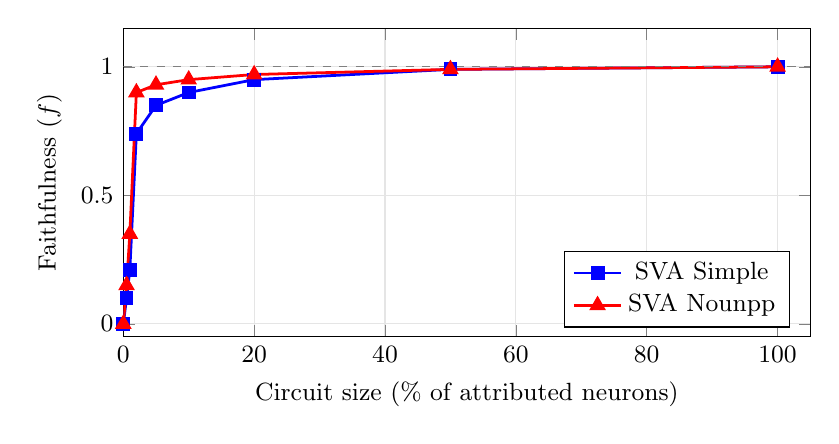
\begin{tikzpicture}
\begin{axis}[
    width=0.85\columnwidth,
    height=5.5cm,
    xlabel={Circuit size (\% of attributed neurons)},
    ylabel={Faithfulness ($f$)},
    xmin=0, xmax=105,
    ymin=-0.05, ymax=1.15,
    legend pos=south east,
    legend style={font=\small},
    grid=major,
    grid style={gray!20},
    tick label style={font=\small},
    label style={font=\small},
]
% SVA Simple
\addplot[
    color=blue, mark=square*, mark size=2pt, line width=1pt,
] coordinates {
    (0, 0.00) (0.5, 0.10) (1, 0.21) (2, 0.74) (5, 0.85) (10, 0.90) (20, 0.95) (50, 0.99) (100, 1.00)
};
\addlegendentry{SVA Simple}

% SVA Nounpp
\addplot[
    color=red, mark=triangle*, mark size=2.5pt, line width=1pt,
] coordinates {
    (0, 0.00) (0.5, 0.15) (1, 0.35) (2, 0.90) (5, 0.93) (10, 0.95) (20, 0.97) (50, 0.99) (100, 1.00)
};
\addlegendentry{SVA Nounpp}

% Reference line at f=1.0
\addplot[dashed, gray, line width=0.5pt] coordinates {(0, 1.0) (105, 1.0)};

\end{axis}
\end{tikzpicture}
\caption{Faithfulness curves on SVA tasks, sweeping percentage thresholds over all attributed neurons with mean ablation. Both curves increase monotonically, with SVA Nounpp achieving $f{=}0.90$ and Simple achieving $f{=}0.74$ at just 2\% of neurons. Dashed line indicates perfect faithfulness ($f{=}1.0$).}
\label{fig:faithfulness}
\end{figure}

\subsection{Edge Attribution and Hourglass Architecture}
\label{sec:edge_results}

\paragraph{Setup.}
We compute edge attribution for the capitals circuit (top 30 target neurons) and refusal circuit, tracing neuron-to-neuron information flow across layers.

\paragraph{Results.}
L23/N8079 emerges as a \emph{double hub}: it receives 172 incoming edges (total weight 977) from earlier layers and sends 38 outgoing edges (total weight 242) to later layers.
This bottleneck structure---where information converges to and diverges from a single neuron---creates an hourglass architecture (Figure~\ref{fig:hourglass}).

\begin{figure}[h]
\centering
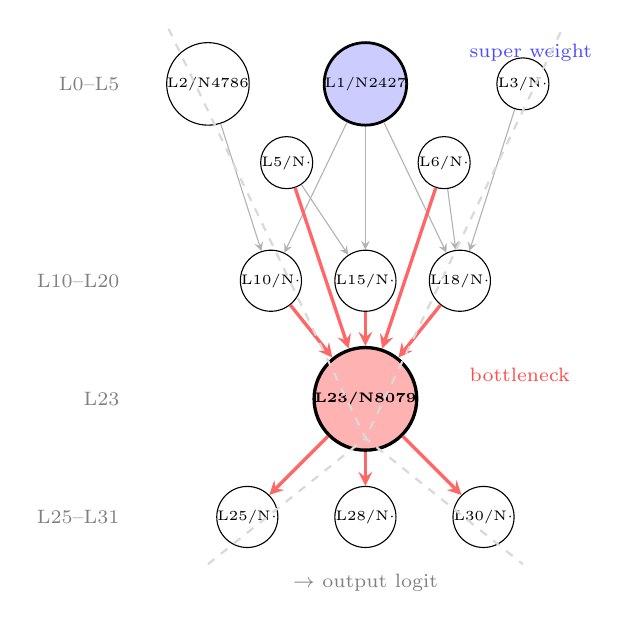
\begin{tikzpicture}[
    neuron/.style={circle, draw, minimum size=6mm, inner sep=0pt, font=\tiny},
    hub/.style={circle, draw, fill=red!30, minimum size=10mm, inner sep=0pt, font=\tiny\bfseries, line width=1.2pt},
    sw/.style={circle, draw, fill=blue!20, minimum size=8mm, inner sep=0pt, font=\tiny, line width=1pt},
    layer/.style={draw=gray!40, dashed, rounded corners, inner sep=4mm},
    arr/.style={->, >=stealth, gray!60},
    harr/.style={->, >=stealth, red!60, line width=1.2pt},
]
% Early layers (wide) — L0-L5
\node[sw] (sw) at (0, 5.5) {L1/N2427};
\node[neuron] (e1) at (-2, 5.5) {L2/N4786};
\node[neuron] (e2) at (-1, 4.5) {L5/N$\cdot$};
\node[neuron] (e3) at (1, 4.5) {L6/N$\cdot$};
\node[neuron] (e4) at (2, 5.5) {L3/N$\cdot$};

% Mid layers (medium) — L10-L20
\node[neuron] (m1) at (-1.2, 3) {L10/N$\cdot$};
\node[neuron] (m2) at (0, 3) {L15/N$\cdot$};
\node[neuron] (m3) at (1.2, 3) {L18/N$\cdot$};

% Bottleneck — L23
\node[hub] (bn) at (0, 1.5) {L23/N8079};

% Late layers (wide) — L25-L31
\node[neuron] (l1) at (-1.5, 0) {L25/N$\cdot$};
\node[neuron] (l2) at (0, 0) {L28/N$\cdot$};
\node[neuron] (l3) at (1.5, 0) {L30/N$\cdot$};

% Edges: early → mid
\draw[arr] (sw) -- (m1);
\draw[arr] (sw) -- (m2);
\draw[arr] (sw) -- (m3);
\draw[arr] (e1) -- (m1);
\draw[arr] (e2) -- (m2);
\draw[arr] (e3) -- (m3);
\draw[arr] (e4) -- (m3);

% Edges: mid → bottleneck (converging)
\draw[harr] (m1) -- (bn);
\draw[harr] (m2) -- (bn);
\draw[harr] (m3) -- (bn);
\draw[harr] (e2) -- (bn);
\draw[harr] (e3) -- (bn);

% Edges: bottleneck → late (diverging)
\draw[harr] (bn) -- (l1);
\draw[harr] (bn) -- (l2);
\draw[harr] (bn) -- (l3);

% Layer labels
\node[anchor=east, font=\scriptsize, gray] at (-3, 5.5) {L0--L5};
\node[anchor=east, font=\scriptsize, gray] at (-3, 3) {L10--L20};
\node[anchor=east, font=\scriptsize, gray] at (-3, 1.5) {L23};
\node[anchor=east, font=\scriptsize, gray] at (-3, 0) {L25--L31};

% Annotations
\node[anchor=west, font=\scriptsize, blue!70] at (1.2, 5.9) {super weight};
\node[anchor=west, font=\scriptsize, red!70] at (1.2, 1.8) {bottleneck};
\node[anchor=north, font=\scriptsize, gray] at (0, -0.6) {$\to$ output logit};

% Hourglass outline
\draw[gray!30, dashed, line width=0.8pt]
    (-2.5, 6.2) -- (0, 1.0) -- (2.5, 6.2);
\draw[gray!30, dashed, line width=0.8pt]
    (-2.0, -0.6) -- (0, 1.0) -- (2.0, -0.6);
\end{tikzpicture}
\caption{Hourglass architecture of the capitals circuit discovered via edge attribution. Information from many early-layer neurons (including the super weight L1/N2427) converges to the bottleneck neuron L23/N8079 (172 incoming edges), which then diverges to late-layer neurons (38 outgoing edges). Node sizes reflect hub degree.}
\label{fig:hourglass}
\end{figure}

\begin{table}[h]
\centering
\caption{Hub analysis for the capitals circuit. Degree = number of edges.}
\label{tab:hubs}
\begin{tabular}{lrrl}
\toprule
\textbf{Neuron} & \textbf{In-degree} & \textbf{Out-degree} & \textbf{Role} \\
\midrule
L23/N8079 & 172 & 38 & Bottleneck (double hub) \\
L1/N2427  & 0   & 38 & Source hub (super weight) \\
\bottomrule
\end{tabular}
\end{table}

L1/N2427, identified as a super weight by the dominance ratio test (4013$\times$ median edge weight), uniformly contributes to both the capitals and refusal circuits with edge weight $-478$, confirming its role as task-agnostic infrastructure.

\subsection{Cross-Model Generalization}
\label{sec:cross_model}

We test our toolkit on Qwen2.5-7B-Instruct and Mistral-7B-Instruct-v0.3 with \emph{zero code changes}.
The architecture-agnostic design (hooking \texttt{model.model.layers[i].mlp.down\_proj}) works across all three model families.

\begin{table}[h]
\centering
\caption{Cross-model generalization. P(``I'') measures refusal probability under circuit ablation. Mistral uses different refusal patterns (lower baseline refusal rate); the P(``I'') metric is not directly applicable.}
\label{tab:cross_model}
\begin{tabular}{lcccc}
\toprule
\textbf{Model} & \textbf{Capitals OK?} & \textbf{P(``I'') normal} & \textbf{P(``I'') ablated} & \textbf{Benign OK?} \\
\midrule
Llama-3.1-8B     & \checkmark & 0.938 & 0.090 & \checkmark \\
Qwen2.5-7B       & \checkmark & 0.975 & 0.025 & \checkmark \\
Mistral-7B-v0.3  & \checkmark & n/a$^\dagger$   & n/a$^\dagger$    & \checkmark \\
\bottomrule
\multicolumn{5}{l}{\footnotesize $^\dagger$ Mistral-7B-v0.3 exhibits different refusal patterns; P(``I'') is not the dominant refusal token.} \\
\multicolumn{5}{l}{\footnotesize \phantom{$^\dagger$} Circuit discovery and capitals steering confirmed functional with zero code changes.}
\end{tabular}
\end{table}

For Qwen, refusal steering works with multiplier sweep: P(``I'') = $0.025 \to 0.816 \to 0.996$ across ablation strengths.
Qwen also reveals its own super weight neurons (L2/N10406 at 4807$\times$ median, L26/N5891 at 5702$\times$ median) via the same automated detection pipeline.


%% ===================================================================
\section{Analysis}
\label{sec:analysis}
%% ===================================================================

\subsection{CAA--RelP Complementarity}

We compare five attribution methods on the capitals task: single-prompt RelP, multi-prompt RelP, residual-stream CAA, MLP-only CAA, and activation-weighted CAA.
L23/N8079 ranks \#1 or \#2 in \emph{all five methods}, making it the most robustly identified circuit neuron.

However, the top-50 overlap between CAA and RelP is only 3--5 neurons out of 50.
This low overlap is \emph{expected}: CAA identifies neurons that are \emph{correlated} with a behavior (high differential activation), while RelP identifies neurons that are \emph{causally responsible} (high attribution flow from output to input).
A neuron can be causally important without having the largest activation difference, and vice versa.
The intersection---neurons that are both correlated and causal---represents the strongest circuit members.

\subsection{Super Weights as Universal Infrastructure}

Edge attribution reveals that super weight neurons (L1/N2427 in Llama, L2/N10406 in Qwen) appear as dominant source hubs in \emph{every} circuit we compute, regardless of task.
Their edge weights are 100--5000$\times$ larger than typical neurons, consistent with the super weight phenomenon described by \citet{zhong2024superweights}.

To our knowledge, this provides the first mechanistic account of super weights within the circuit framework: they are not task-specific computational elements but rather \emph{universal infrastructure neurons} whose anomalously large activations propagate through every downstream computation.
Our blacklisting procedure automatically detects and excludes them, preventing inflation of task-specific circuits.

\subsection{Steering Precision}

A key advantage of neuron-level steering over residual-stream methods (CAA, representation engineering) is \emph{specificity}.
Ablating the refusal circuit changes only the safety behavior; factual knowledge, coherence, and language quality are preserved.
This is because neuron steering modifies ${\sim}200$ out of ${\sim}460{,}000$ MLP neurons (0.04\% of the model), compared to CAA which modifies the entire residual stream at one or more layers.


%% ===================================================================
\section{Related Work}
\label{sec:related}
%% ===================================================================

\paragraph{Circuit discovery.}
Automated Circuit Discovery (ACDC) \citep{conmy2023acdc} and path patching \citep{goldowskydill2023localizing} identify circuits via iterative edge pruning, but require many forward passes.
Interchange intervention \citep{geiger2024interchange} provides causal guarantees but is similarly expensive.
Our RelP-based approach achieves comparable circuit quality in a single forward-backward pass.

\paragraph{Sparse autoencoders.}
SAEs \citep{cunningham2023sae, bricken2023monosemanticity, templeton2024scaling} learn interpretable features via unsupervised dictionary learning.
Sparse Feature Circuits \citep{marks2024sparse} use SAEs for circuit discovery.
These methods require expensive training and face the granularity trade-off: too few features miss structure, too many create redundancy.
Neuron-basis circuits sidestep this entirely---the ``dictionary'' is the model's own neurons.

\paragraph{Representation engineering.}
CAA \citep{rimsky2024steering} and representation engineering \citep{zou2023representation} steer models via residual-stream modifications.
Our neuron-level steering achieves similar behavioral effects with higher specificity (0.04\% of model vs.\ full residual stream).

\paragraph{Mechanistic interpretability.}
The Indirect Object Identification circuit \citep{wang2023ioi} and subsequent work on grokking \citep{nanda2023progress} have demonstrated that specific model behaviors can be understood as circuits.
Our toolkit makes this style of analysis accessible for any behavior expressible as a prompt or prompt contrast.


%% ===================================================================
\section{Limitations}
\label{sec:limitations}
%% ===================================================================

\textbf{Linearization approximation.}
The three LRP rules introduce approximation error by treating non-linear components (RMSNorm, SiLU sigmoid, attention softmax) as locally linear.
While \citet{arora2025circuits} demonstrate 0.956 correlation between RelP and activation patching, the approximation may be less accurate for models with very different non-linearities.

\textbf{Single-token attribution.}
Our pipeline attributes toward a single target token.
Multi-token behaviors (e.g., extended reasoning chains) require either sequential single-token attribution or aggregation strategies not yet validated.

\textbf{Position dependence.}
Circuit neurons are identified at specific token positions.
Our steering hooks apply across all positions during generation, which is an approximation; the causal role of a neuron may differ across positions.

\textbf{Model family scope.}
We demonstrate generalization across Llama, Qwen, and Mistral families, all of which use the same gated-MLP architecture ($\text{SiLU}(\text{gate}) \times \text{up}$).
Models with different MLP architectures (e.g., standard ReLU MLPs, mixture-of-experts) would require modified linearization rules.

\textbf{Contrastive circuits lack faithfulness evaluation.}
Our contrastive discovery method (Section~\ref{sec:contrastive}) operates on raw activation differences rather than RelP attribution, so the standard faithfulness metric (which requires attribution scores and percentage thresholding) does not directly apply.
We evaluate contrastive circuits only via behavioral steering (P(``I'') shift, benign preservation), not via the faithfulness/completeness metrics used for RelP-discovered circuits.

\textbf{MLP linearization variant.}
Our Half-rule implementation uses detached sigmoid plus 50/50 gradient split (following the RelP formulation), while the TransluceAI codebase defaults to full gate detachment (\texttt{StopGradGateMLP}).
Both are valid linearizations of the gated MLP, but they produce slightly different attribution scores.
We verified correctness against the RelP formulation; exact reproduction of TransluceAI's default attributions would require switching to their gate-detach variant.

\textbf{Evaluation scope.}
Our faithfulness evaluation focuses on SVA and factual recall.
Broader evaluation on reasoning, multi-step tasks, and more diverse behavioral steering would strengthen the claims.


%% ===================================================================
\section{Conclusion}
\label{sec:conclusion}
%% ===================================================================

We have presented a practical toolkit for neuron-level circuit discovery and steering in large language models.
By implementing the three LRP rules (LN-rule, AH-rule, Half-rule) in a single-file Python module, we make it possible to discover faithful circuits in a single forward-backward pass, steer model behavior by modifying ${\sim}200$ neurons (0.04\% of the model), and trace neuron-to-neuron information flow---all with zero external interpretability dependencies.

Our key findings are:
(1) As few as 2\% of attributed neurons achieve faithfulness $f{=}0.74$--$0.90$ on syntactic agreement tasks (varying by task complexity).
(2) Contrastive circuit discovery identifies ${\sim}200$ neurons responsible for safety refusal, and their ablation converts refusal to compliance while preserving benign behavior.
(3) Edge attribution reveals an hourglass architecture with bottleneck neurons serving as information routing hubs.
(4) Super weight neurons are detectable as universal infrastructure via edge attribution, providing what is, to our knowledge, the first connection between super weights and mechanistic circuit analysis.
(5) The entire approach generalizes across model families with zero code changes.

Neuron-basis circuit analysis represents a practical middle ground between expensive SAE-based methods and coarse residual-stream interventions.
We release our toolkit to enable broader adoption of mechanistic interpretability in both research and safety applications.


\bibliography{references}
\bibliographystyle{plainnat}

\newpage

%% ===================================================================
\appendix
\section{Toolkit API Reference}
\label{sec:api}
%% ===================================================================

The toolkit is distributed as a single Python file \texttt{neuron\_steer.py} with no dependencies beyond PyTorch and Hugging Face Transformers.
The primary interface is the \texttt{NeuronSteerer} class:

\begin{verbatim}
from neuron_steer import NeuronSteerer

# Initialize (auto-detects universal neurons)
s = NeuronSteerer("meta-llama/Llama-3.1-8B-Instruct")

# Discover circuit for factual recall
circuit = s.discover_circuit(
    "What is the capital of Texas?", " Austin",
    top_k=200
)

# Steer: ablate circuit neurons
output = s.steer_and_generate(
    "What is the capital of Texas?",
    circuit, multiplier=0.0
)

# Contrastive discovery for refusal
refusal = s.discover_contrastive(
    positive_prompts=harmful_prompts,
    negative_prompts=benign_prompts,
    top_k=200
)

# Edge attribution
graph = s.discover_edges(
    "What is the capital of Texas?", circuit
)
print(graph.summary())
print(graph.detect_super_weights())

# Faithfulness evaluation
data = s.measure_faithfulness_batch(
    prompts, targets, counterfactuals,
    attributions=raw_attrs
)
\end{verbatim}

\section{Hard-Coded Universal Neuron Blacklist}
\label{sec:blacklist_appendix}

For Llama-3-8B, the following 12 neurons are hard-coded from the TransluceAI codebase as universal (task-independent) and excluded from all circuits:

\begin{center}
\begin{small}
\begin{tabular}{cccccc}
\toprule
L2/N4786 & L5/N7012 & L6/N5866 & L7/N6673 & L9/N4255 & L10/N11570 \\
L11/N11321 & L13/N4208 & L16/N1241 & L18/N7417 & L20/N3972 & L23/N306 \\
\bottomrule
\end{tabular}
\end{small}
\end{center}

For other architectures, the automated detection procedure (Section~\ref{sec:blacklist}) generates model-specific blacklists.

\section{Experimental Details}
\label{sec:exp_details}

\paragraph{Hardware.}
All experiments run on NVIDIA B200 GPUs (180\,GB HBM3e) with CUDA 12.x.
Models are loaded in bfloat16 precision.

\paragraph{Hyperparameters.}
Unless stated otherwise: percentage threshold $\tau{=}0.005$, top-$k$ per layer for attribution $= 200$, BOS position filtered, eager attention enabled.
Faithfulness evaluation uses left-padded batching with mean ablation.

\paragraph{Prompts.}
Capital city prompts follow the pattern ``What is the capital of the state containing [City]?'' with seed response ``Answer:''.
The 10 training city--capital pairs are listed in Table~\ref{tab:training_pairs}.
Held-out evaluation uses Pittsburgh $\to$ Harrisburg, Houston $\to$ Austin, and one additional pair.
Refusal prompts are drawn from standard safety benchmarks.
SVA prompts use the format from \citet{arora2025circuits}.

\begin{table}[h]
\centering
\caption{Training city--capital pairs for the factual recall task.}
\label{tab:training_pairs}
\begin{tabular}{ll}
\toprule
\textbf{City in prompt} & \textbf{Target capital} \\
\midrule
Dallas       & Austin \\
Phoenix      & Phoenix \\
Miami        & Tallahassee \\
Seattle      & Olympia \\
Portland     & Salem \\
Denver       & Denver \\
Chicago      & Springfield \\
Detroit      & Lansing \\
Atlanta      & Atlanta \\
San Diego    & Sacramento \\
\bottomrule
\end{tabular}
\end{table}

\end{document}
